% Created 2021-03-14 Sun 16:03
% Intended LaTeX compiler: pdflatex
\documentclass[11pt]{article}
\usepackage[utf8]{inputenc}
\usepackage[T1]{fontenc}
\usepackage{graphicx}
\usepackage{grffile}
\usepackage{longtable}
\usepackage{wrapfig}
\usepackage{rotating}
\usepackage[normalem]{ulem}
\usepackage{amsmath}
\usepackage{textcomp}
\usepackage{amssymb}
\usepackage{capt-of}
\usepackage{hyperref}

\date{\today}
\title{Entropy in Evolutionary Algorithms}
\author{Lucas Blakeslee\footnote{\texttt{lqblakeslee@gmail.com}},
  Aengus McGuinness\footnote{\texttt{aengus82520@gmail.com}}}
\hypersetup{
 pdfauthor={},
 pdftitle={},
 pdfkeywords={},
 pdfsubject={},
 pdfcreator={Emacs 27.1 (Org mode 9.3)}, 
 pdflang={English}}

\begin{document}
\maketitle
%% \tableofcontents


\label{sec:org26f53e0}
\begin{abstract}
\label{sec:orga17da23}

Genetic algorithms (GAs) are an optimization technique inspired by
natural selection. GAs have yielded good results in certain practical
problems, yet there is still more to be understood about their
behavior on a theoretical level. One approach is to look at the
evolutionary process from the point of view of statistical mechanics,
and interpreting jumps in fitness as phase transitions. Toward this
goal we examine the behavior of \emph{entropy} in a GA that optimizes
a simple function.  We find that entropy increases as a new species
diversifies, but its upper bound decreases with most phase
transitions (which correspond to evolutionary steps).
\end{abstract}


%% -\textbf{- mode: org -}-


\section{Motivation:}
\label{sec:org16abecd}
Genetic algorithms (GAs) are stochastic search algorithms based on the
process of natural evolution, solving for the 'fittest' solutions to a
problem. GAs are optimization algorithms, designed to maximize or
minimize certain functions. GAs are much more efficient than random or
exhaustive search algorithms (Kinnear, 1994), however, they do not
scale well with complexity (Radcliffe \& Surry, 1995). While specifics
may vary, there are some processes universal to GAs, which are:
population → fitness evaluation → selection → crossover → mutation,
repeat. Each organism in the population has its own 'chromosome,' or
set of characteristics. Here is where the resemblance to biological
evolution begins to weaken. The process continues to occur either
until some condition for termination has been met, or until a
pre-specified number of iterations has elapsed. Genetic algorithms
have been used in a variety of practical applications, from making
"evolved antennae" for spacecrafts and satellites to the estimation of
heat flux between sea ice and the atmosphere to predictive economic
models. Entropy and evolution have been often explored together, with
research on the subject going as far back as the 1870s, though
Schrödinger's 1944 book \emph{What is life?} sparked a wave of modern
interest. Here it was wondered how entropy would change over time in a
genetic algorithm, in order to attain a better theoretical grasp of
how they function.

\section{Hypothesis:}
\label{sec:org26a3be1}
It was hypothesized that entropy would gradually rise as small non-significant mutations arose, and the occurance of one highly beneficial mutation in an organism would cause entropy to rapidly decrease as that mutation was selected for, and then entropy would continue to rise, and the same cycle would repeat. It was hypothesized that the entropy would never again become as high as it was originally. One "iteration" of this hypothesized cycle would look like a backwards log normal distribution.

\section{Approach:}
\label{sec:org8c588e5}
A plan was made, involving first construct a relatively simple genetic algorithm, and then analyzing the ways in which entropy changes over the course of finding a solution. The way that was decided to do this was to track diversity as a means of measuring the entropy.

\section{Methods:}
\label{sec:org2c55902}
First, a simple genetic algorithm was constructed to find the maxima of a polynomial, using the IEEE 754 floating point format to represent the chromosomes of the organisms, or that organism's coefficients of X. The polynomial was structured as: ax\textsuperscript{7} + ax\textsuperscript{6}  \ldots{} + ax\textsuperscript{2} + ax + a.

The population of 10,000 underwent the standard evalutation, selection, crossover, and mutation of a  GA, with information about the population being collected at the end of each iteration. Diversity was measured using the hamming distance between the binary strings of two organisms, and the Shannon entropy of the population was calculated at the end of each iteration. Additionally, the elite and average fitnesses of the population were tracked.

\section{Results:}
\label{sec:orged0917a}
[I'm a little unclear on what our actual results were]


\begin{figure}
  \centering{}
  \resizebox{0.5\linewidth}{!}{%
    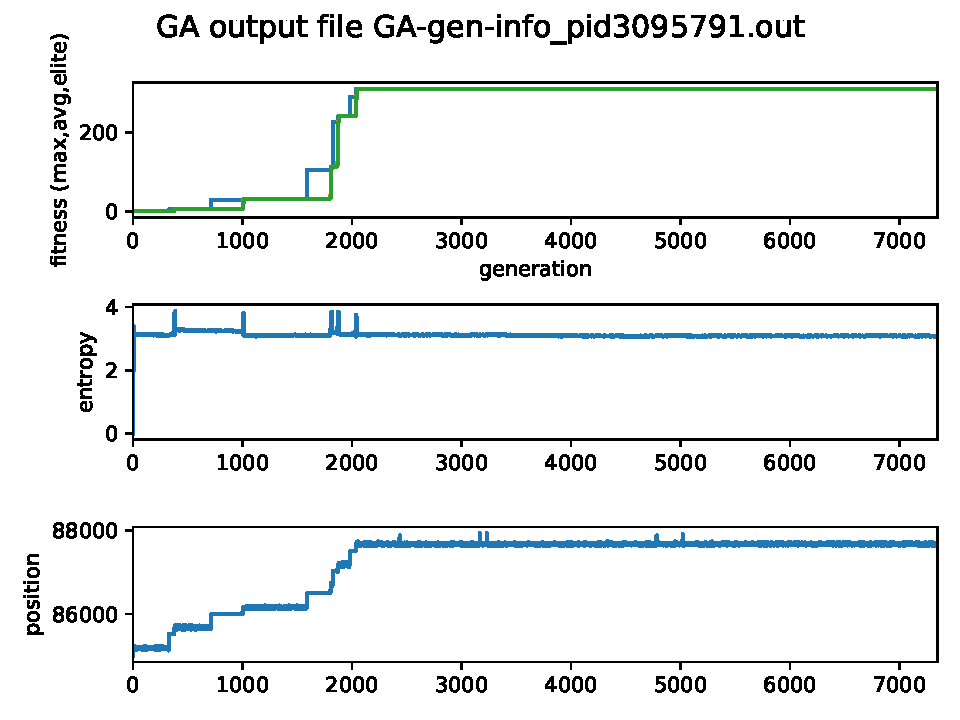
\includegraphics{GA-gen-info_pid3095791.out.pdf}
  }
  \caption{One example of evolution FIXME add more.}
  \label{fig:multi-step}
\end{figure}

\begin{figure}
\end{figure}

\section{Discussion:}
\label{sec:org7999995}
\subsection{what does this mean?}
\label{sec:orgf7b36ed}
[once we have concrete results we can delve into this]

\subsection{Limitations to genetic algorithms}
\label{sec:org148bf83}
There are some limitations to genetic algorithms. For example, one must have a very clear understanding of the problem, constraints, the data structure, etc. Additionally, genetic algorithms do not scale well with complexity -- problems with large numbers of elements often become exponentially more difficult to compute. There is also the difficulty of ensuring the algorithm doesn't get stuck on a local maxima rather than the global one.

\subsection{Future work}
\label{sec:org0f04af1}
Going forwards, it could be interesting to optimize a genetic algorithm from the standpoint of its entropy.

\section{References}
\label{sec:org9dc046e}
\textbf{these will ultimately need to be alphebatized by last name of the first author} \textbf{the citation style should be consistent, I was thinking APA}

Kinnear, K. E. (1994). In K. E. Kinnear (Ed.), \emph{Advances in Genetic Programming} (pp. 3-17). Cambridge: MIT Press.

Radcliffe N.J., Surry P.D. (1995) Fundamental limitations on search algorithms: Evolutionary computing in perspective.
In: van Leeuwen J. (eds) Computer Science Today. Lecture Notes in Computer Science, vol 1000. Springer, Berlin, Heidelberg.
\url{https://doi.org/10.1007/BFb0015249}
\end{document}
